\documentclass{article}

\usepackage[margin=1in]{geometry}
\usepackage{color}
\usepackage{hyperref}
\usepackage{soul}
\usepackage{float}
\usepackage{amsmath}

\usepackage[sc]{mathpazo}
\linespread{1.20}         % Palatino needs more leading (space between lines)
\usepackage[T1]{fontenc}
\usepackage{microtype}
\usepackage{listings}
\usepackage{courier}
\usepackage{graphicx}

\definecolor{mygreen}{rgb}{0,0.6,0}
\definecolor{light-gray}{gray}{0.95}

\lstset{basicstyle=\footnotesize\ttfamily,breaklines=true,language=Prolog}
\lstset{frame=single,commentstyle=\color{mygreen}}
\lstset{aboveskip=0.5cm,belowskip=0.3cm}
\lstset{backgroundcolor=\color{light-gray}}

\hypersetup{pdfpagemode=UseNone}

\newcommand{\manager}{\texttt{manager} }
\newcommand{\eagent}{\texttt{elevator agent} }
\newcommand{\eagents}{\texttt{elevator agents} }
\newcommand{\todo}[1] {\hl{TODO: #1}}
\newcommand{\horrule}[1]{\rule{\linewidth}{#1}}
\setlength{\parindent}{0cm}

\title{ 	
		\usefont{OT1}{bch}{b}{n}
		\normalfont \normalsize \textsc{Delft University of Technology \protect\\ Data Visualization 2015 - 2016} \\ [25pt]
		\horrule{0.5pt} \\[0.4cm]
		\huge Football Match Visualization Project \\
		Individual Report
		\horrule{2pt} \\[0.5cm]
}
\author{
		\normalfont 								\normalsize
        Overvoorde Alexander 4153235\\[-3pt]		\normalsize
        \today
}
\date{}
\begin{document}
\lstset{language=Prolog}
\maketitle

\newpage

\section{3D visualization}

I wrote a Python script that took the position, energy and speed data and generated team and per-player heatmaps from these as 2D grids with values scaled from 0 to 1. I visualized these with three.js for the 3D visualization (figure \ref{fig:3dvis}) by creating a plane and deforming it based on the heatmap value. The color is calculated using a d3.js scale. For the field I created the models (pitch, goals) with Blender. The positions of players are taken directly from the 2D visualization, so they indirectly use d3.js interpolation.

\begin{figure}[ht!]
    \centering
    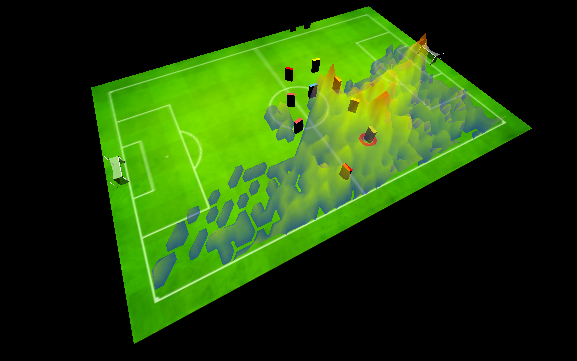
\includegraphics[scale=0.55]{3dvis.png}
    \caption{3D visualization with heatmap}
    \label{fig:3dvis}
\end{figure}

\section{2D visualization}

I also developed the 2D visualization (figure \ref{fig:2dvis}) with d3.js and wrote the code for the playback controls and heatmap selection. The heatmap selection toggles the "visible" property of the generated heatmap meshes in the three.js visualization. The play/pause button and playback speed selector modifies the frequency of a timer that loads the next frame of player positions. The updates use d3.js transitions to make movement appear smoothly.

\begin{figure}[ht!]
    \centering
    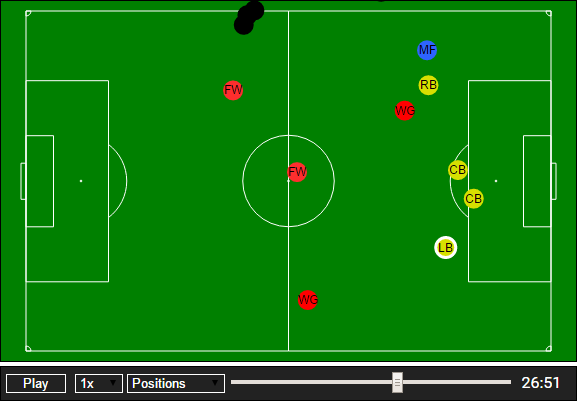
\includegraphics[scale=0.55]{2dvis.png}
    \caption{2D visualization with playback controls}
    \label{fig:2dvis}
\end{figure}

\end{document}